\chapter{Integración en sistemas CI/CD}\label{sec:cicd}

\paragraph{}Cuando hablamos de sistemas \gls{CI/CD} nos solemos referir a todos aquellos
servidores, servicios y máquinas; ya sean \gls{on premises} o en cloud, que posibilitan
el desarrollo centralizado, el control de versiones, el aseguramiento de la calidad
y la entrega continua.

\paragraph{}\textbf{Nota: }\emph{Cómo entrar en detalle en estos apartados sería extender
demasiado el alcance que se prentende en este trabajo, este capítulo se va a limitar a
describir la relación del entorno de desarrollo con los sistemas \gls{CI/CD}. Cualquier
arquitectura de la infraestructura es pura expeculación y no será probada a nivel práctico.}

\section{Control de versiones}

\paragraph{}El control de versiones en este entorno de desarrollo se realiza mediante
\gls{git}. \Gls{git} es una herramienta de control de versiones gratuita, multiplataforma que
es muy popular, tanto que incluso podría empezar a considerarse un estandar. Populares
servicios de repositorios online, como \href{github.com}{github} o \href{gitlab.com}{gitlab}
funcionan con este sistema. Para este proyecto, se ha elegido \href{github.com}{github}
por su popularidad. Ya que al ser código abierto, esto facilita que más desarrolladores
encuentren el proyecto e incluso quieran colaborar para hacer sus aportaciones.

\paragraph{}En mi experiencia laboral, he utilizado \gls{git} en repositorios compartidos
por más de mil desarrolladores y \gls{git} facilita la gestión del control de versión.
Obviamente, en casos tan ``extremos'' como el mencionado, existen carencias que no
resuelve la propia herramienta, y que han de ser solventados mediante la implantación
de protocolos internos y patrones de branching.

\paragraph{}Algunos de los patrones más utilizados son: patrón mainline branch, healthy
branch, feature branch, release branch o production branch. Estos patrones deben ser
implementados en función de la naturaleza del proyecto, se la cantidad de cambios que
sufre el código, la metodología de desarrollo de la empresa, de la relación con el
cliente, etc.

\subsection{} Ciclo de vida del desarrollo software

\paragraph{}Yocto admite tener tanto fuentes locales, como fuentes en servidores. Por
eso mismo, para el desarrollo de la aplicación flutter se propone el uso de los
siguiente patrones de branching, explicando sus fundamentos.

\begin{figure}[H]
    \centering
    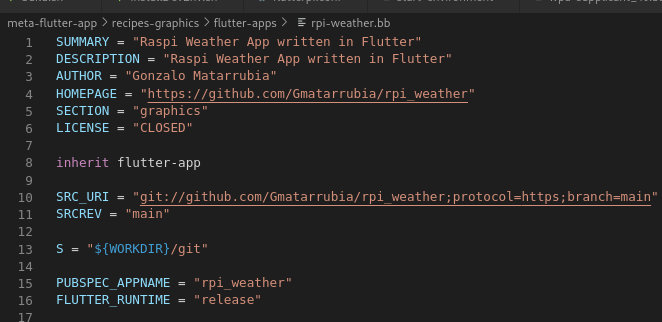
\includegraphics[width=0.90\textwidth]{imgs/rpi-weather-recipe}
    \caption[Detale recipe de Rpi Weahter]{Detalle de la recipe de Rpi Weather.}
    \label{imgs:recipe-rpi-weather-1}
\end{figure}

\paragraph{}Como se puede apreciar en la imagen \ref{imgs:recipe-rpi-weather-1} cada
vez que se haga un \gls{fetch} de Rpi Weather, va a descargar lo último que haya en la
rama principal. Esto tiene unas consecuencias inmediatas. La rama principal debe contener
en todo momento código funcional dispuesto a ser entregado y que pase todas las pruebas
necesarias. En un entorno real, lo más conveniente sería fijar la referencia de una recipe,
o bien a un \emph{tag} o \emph{commit} concretos o bien a una rama de release. Pero para
nuestro ejemplo, vamos a considerar la rama \emph{main} como una rama de release.

\paragraph{Patrón de always-ready main branch:} blabla

\paragraph{Patrón de healthy branch:} blabla

\paragraph{Patrón de feature branch:} blabla

\paragraph{}Al no haber otro proyecto que depende del código del entorno Yocto, para
esta parte podría haber una política de branching diferente, posiblemente más relajada.
Pero al pertenecer ambos entornos, el de Flutter y el de Yocto a la misma compañia, se
aplicará extamente la misma política de branching, así se homogenizan los procesos.

\subsection{} Infraestructura

\paragraph{}Normalmente, los sistemas de control de versiones están ``supervisados''
por equipos de compilación, analizadores estáticos y dinámicos, despligue de artefactos,
etc. Es decir, que existe una infraestructura que trabaja de forma automatizada con
nuestro código y los cambios que le introducimos. Esta infraestructura puede estar
en local, \gls{on premises} o en cloud. Lo único que cambia en cada caso es la hubicación
física del \emph{hardware}, así como la responsabilidad de mantener el servicio.

\paragraph{}Para asegurar la mantenibilidad de esta infraestructura, así como para aplicar
las mismas técnicas de desarrollado que se hacen con el código se llevan a cabo descripciones
de \glsplural{pipeline} en lo que se conoce como \gls{IaaC}. De esta manera, el desarrllo
del entorno de desarrollo y sus dependencias puede ser desarrollado y administrado a la
vez y de igual manera que el propio código que contiene.



\section{QA}

\paragraph{}Blabla

\section{Entrega continua}

\paragraph{}Blabla

%las referencias a artculos se ponen con \cite,
%las referencias a imgenes \ref,
%las referencias a glosario \gls,
%y las referencias a ecuaciones \eqref
